\chapter{Projektstrukturplan}
%Erstellen eines Projektstrukturplans für das Digitalisierungsprojekt
%− Auswahl und Begründung einer Zerlegungsart für den PSP
%− Beschreibung der Arbeitspakete mit den gängigen Elementen
%(die Arbeitspakete können auch als User Stories nach INVEST-Prinzip beschrieben werden)
%− Keep it simple
%− Analog Szenario 1: Datei „1_Basis“ verwenden
\label{chapter:2}


Für das Projekt Operation-Digipaper wurde auf Grundlage des bereitgestellten Szenarios und dem daraus abgeleiteten Projektsteckbrief ein Projektstrukturplan mit den wichtigsten Arbeitspaketen entworfen. Aus dem Szenario für das Projekt ergibt sich eine gewisse Komplexität aber um die Ausarbeitung in einem angemessenen Rahmen zu halten, wurde in dieser Gruppenarbeit die Anzahl der Arbeitspakete auf 12 Stück reduziert. Es wurden daher teils Einzelarbeitsschritte zu größeren Paketen zusammengefasst. Es sind alle wichtigen Aspekte des Projektes enthalten, die für eine erfolgreiche Umsetzung der Digitalisierungsmaßnahmen bei der CP Service GmbH notwendig sind. 


\section{Gliederung des Projektes}

Bei der Erstellung des Projektstrukturplans wurde sich für eine phasen- bzw. zeitorientierte Gliederung entschieden, da sich das Projekt perfekt in 5 Phasen gliedern lässt, welche sequentiell aufeinander folgen müssen und inhaltlich überschneidungsfrei sind. 

%Bei der Erstellung des Projektstrukturplans wurde sich für eine phasen- bzw. zeitorientierte Gliederung entschieden, da sich das Projekt perfekt in 5 Phasen einteilen lässt. Die Arbeitsabschnitte müssen sequentiell aufeinander folgen und sind inhaltlich überschneidungsfrei. Da bei einer phasenorierntierten Gliederung jede Phase eindeutige, klar definierte Aufgaben beinhaltet, welche erst abgeschlossen werden müssen, bevor die nächste Phase beginnt, ist diese Gliederung somit für das Projekt gut geeignet.

So lässt sich der Projektverlauf in eine Konzeptionierungs-, Entwicklungs-, Testing-, Pilotierung- sowie eine Rollout-Phase unterteilen. Welche Arbeitspakete hierbei in den einzelnen Phasen zu bearbeiten sind, ist Abbildung 2.1 zu entnehmen.


%Bei der Erstellung des Projektstrukturplans wurde sich für eine phasen- bzw. zeitorientierte Gliederung entschieden, da diese gut mit dem Umfang und Zielen des Projektes vereinbar ist. Neben der eigentlichen Softwareentwicklung, scheint noch konzeptionelle Arbeit notwendig und besonders die Anforderung einer Pilotierungsphase und die hohen Testansprüche wurden als wichtig beurteilt. Die einzelnen Teilbereiche bauen aufeinander auf und lassen sich in separierbare Phasen gliedern.

%Von einer objektorientierten Zerlegung wurde abgesehen, da die Anforderungen an die neue Softwarekomponente überschaubar sind und sich somit nur wenige Teilobjekte ergeben hätten. 

%Auch die funktionsorientierte Zerlegung hat sich für dieses Projekt nicht durchgesetzt, da bei dem Großteil der Aufgaben zumindest eine Teil-Entwicklungsfunktion von Bedeutung ist, und keine anderen größeren Funktionsbereiche abgrenzt werden konnten.

%Die phasenorientierte Zerlegung ermöglicht es besonders die zeitlichen Abgrenzungen im Projektverlauf in den Vordergrund zu stellen, welches aufgrund der Dringlichkeit des Projektes und der vorgegebenen dreimonatigen Pilotierungsphase letztendlich mit ausschlaggebend bei der Gliederungswahl war. Letztendlich wurden folgende Phasen beschlossen: Konzeptionierung, Entwicklung, Testing, Pilotieren, Rollout. Diese sind zusammen mit ihren jeweiligen Arbeitspaketen in Abbildung \ref{fig:PSP} dargestellt.

%Auch die funktionsorientierte Zerlegung hat sich für dieses Projekt nicht durchgesetzt, da sich das Projekt auf ein Scrum Team mit 8 Personen beschränkt, welche zum Großteil in einer Entwicklungsfunktion tätig sind. Andere typische Funktionsbereiche wie 


%Von einer objektorientierten Zerlegung wurde abgesehen, da die Anforderungen an die neue Softwarekomponente überschaubar sind und auch keine 


% gegen funktionalität: scrum team aus 8 leuten deckt nicht zwingend funktionen ab die abzugrenzen sind. entwickler können mehrere sachen machen --> entwicklung ist die eine hauptfunktion und sachen wie Vertrieb, Marketing, also andere funktionen spielen nur eine nebengeordnete rolle
% gegen objekt: anforderungen sind überschaubar und es sollen nicht in kleine objekte unterteilt werden / (objekte sind nur für dieses projekt und nicht übergreifend) einzelobjekte welche nicht wiederverwendet werden würden


%Beim Erstellen des Projektstrukturplans wurde das Gegenstromverfahren angewendet. Es wurde somit erst deduktiv (Top-Down) gearbeitet und dann induktiv (Bottom-Up) Verbesserungen durchgeführt. Dieses wurde im Wechsel fortgeführt und so ein vollständiger und realistischer Projektstrukturplan ausgearbeitet.

\begin{figure}[H]
	\centering
	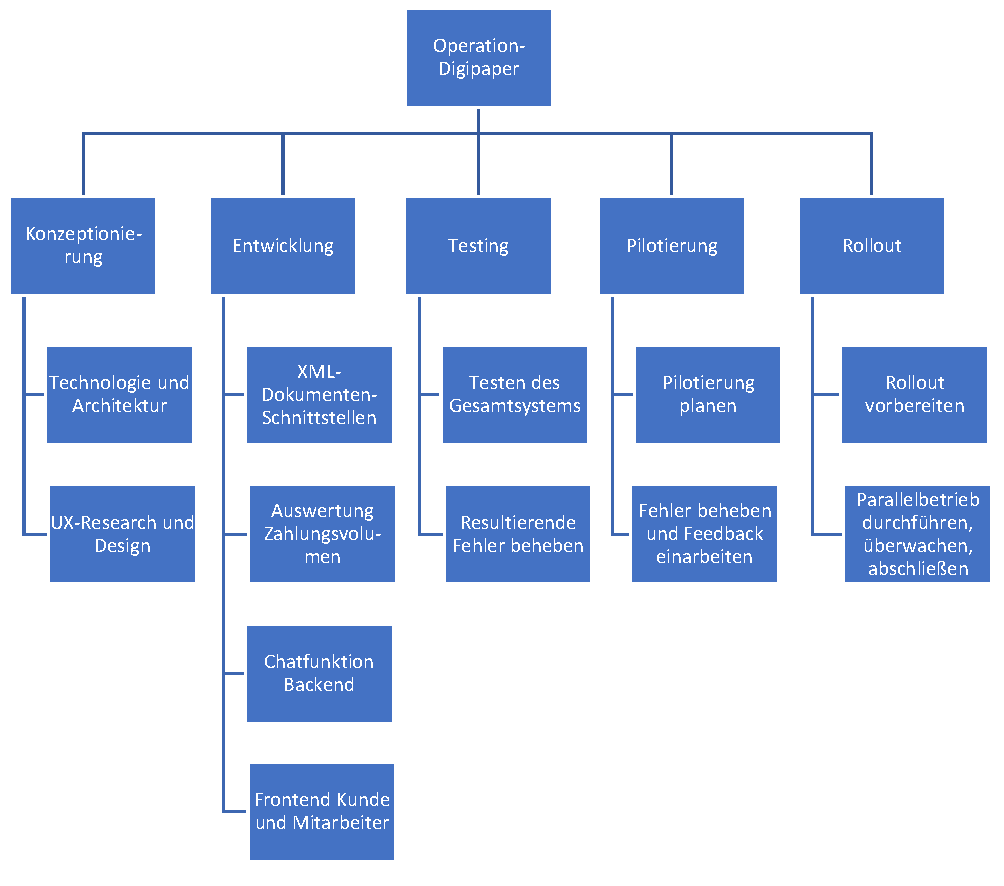
\includegraphics[width=\linewidth] {img/PSP.pdf}
	\caption{Projektstrukturplan}
	\label{fig:PSP}
\end{figure}

\section{Arbeitspakete}

Im Folgenden findet sich die Ausarbeitung der zuvor festgelegten Arbeitspakete. Es wurden die gängigen Elemente zur Beschreibung eines Arbeitspaketes genutzt und besonders die Aufgabenstellung in den Vordergrund gestellt. 

Der geplante Aufwand basiert auf den in Kapitel \ref{chapter:3} mittels Planning-Poker bestimmten Storypoints. Das Team arbeitet sehr produktiv und die Dauer kann daher aus einer 1:1 Umrechnung der Storypoints in Tage angesetzt werden.
Als Verantwortliche wurden jeweils Personen aus dem in Kapitel \ref{chapter:4} bestimmten Scrum-Team gewählt.

%Die Risiken sind mit den in Kapitel \ref{chapter:4} aufgeführten Beispielen abgestimmt.
\newpage
% --- Konzeptionierung ---

\textbf{Konzeptionierung}\newline
In der ersten Projektphase werden die technologischen und designorientierten Grundlagen für das Projekt geschaffen. Sie umfasst die Identifizierung geeigneter Technologien und den Entwurf einer Architektur für die zu entwickelnde Software. Dies wird durch eine umfangreiche Benutzerforschung und Designarbeit ergänzt.


\phantomsection
\begin{xltabular}{\textwidth}{|>{\hsize=.3\hsize}X|>{\hsize=.7\hsize}X|}
	\hline
	\textbf{PSP-Code} & 
	\textbf{AP-K-1} \\
	\hline
	Name AP & 
	Technologie und Architektur\\
	\hline
	Verantwortlicher & 
	Anna Schmidt\\
	\hline
	Aufgabenstellung & 
	Die zu erfüllenden Aufgaben umfassen die Identifizierung geeigneter Technologien für das Projekt und die Erstellung einer entsprechenden Technologieliste. Anschließend muss eine Architektur für die zu entwickelnde Software entworfen werden.\\
	\hline
	Zieldefinition & 
	Es wurde eine vollständige Technologieliste entworfen und die Architektur dokumentiert.\\
	\hline
	Voraussichtliche Dauer & 6,5 Tage\\
	\hline
	Voraussetzungen & Projektauftrag erteilt\\
	\hline
	Geplanter Aufwand & 6,5\\
	\hline
	Hilfsmittel & \\
	\hline
	Risiken & 
	Technologische Innovation führt dazu, dass Lösung bis zum Projektabschluss bereits veraltet ist\\
	\hline
	Evtl. Schnittstellen & \\
	\hline
	Abnahmebedingungen & 
	Abnahme durch Projektleiter und Leiter der IT-Abteilung\\
	\hline
\end{xltabular}
\addcontentsline{lot}{table}{2.1 \ \ AP Technologie und Architektur}
\label{tab:my_label1}

\newpage
\phantomsection
\begin{xltabular}{\textwidth}{|>{\hsize=.3\hsize}X|>{\hsize=.7\hsize}X|}
	\hline
	\textbf{PSP-Code} & 
	\textbf{AP-K-2}\\
	\hline
	Name AP & 
	UX-Research und Design\\
	\hline
	Verantwortlicher & 
	Susi Sonnenschein\\
	\hline
	Aufgabenstellung & 
	Es sollen Personas entworfen und Interviews mit Stakeholdern geführt werden, um Customer Journey Maps zu erstellen. Im Anschluss daran gilt es, Wireframes zu entwerfen und deren Design durch Nutzertests zu validieren.\\
	\hline
	Zieldefinition & 
	Eine Designspezifikation wurde entworfen und an die Entwickler (Leiter der IT-Abteilung) übergeben.\\
	\hline
	Voraussichtliche Dauer & 14,75 Tage\\
	\hline
	Voraussetzungen & Projektauftrag erteilt\\
	\hline
	Geplanter Aufwand & 14,75\\
	\hline
	Hilfsmittel & 
	Projektstrukturbrief (Ziel, Inhalt und Abgrenzung)\\
	\hline
	Risiken & 
	Missachtung der Wünsche und Anforderungen von Kunden führt zu fehlender Akzeptanz der Lösung\\
	\hline
	Evtl. Schnittstellen & \\
	\hline
	Abnahmebedingungen & 
	Übergabe von Entwicklern bestätigt und Abnahme durch Projektleiter\\
	\hline
\end{xltabular}
\addcontentsline{lot}{table}{2.2 \ \ AP UX-Research und Design}
\label{tab:my_label2}

% --- Entwicklung ---
\newpage
\textbf{Entwicklung}\newline
In der Entwicklungsphase des Projekts erfolgen die tatsächlichen Implementierungsarbeiten. Dies umfasst das Programmieren der geplanten Schnittstellen und der Zahlungsauswertung. Es wird zudem eine Chatfunktion geschaffen und auf Grundlage dieser Backend-Elementen das Frontend umgesetzt.

\phantomsection
\vspace{-0.8mm}
\begin{xltabular}{\textwidth}{|>{\hsize=.3\hsize}X|>{\hsize=.7\hsize}X|}
	\hline
	\textbf{PSP-Code} & 
	\textbf{AP-E-1}\\
	\hline
	Name AP & 
	XML-Dokumenten-Schnittstelle\\
	\hline
	Verantwortlicher & 
	Harry Mayer\\
	\hline
	Aufgabenstellung & 
	Die Aufgaben beinhalten die Entwicklung einer XML-Schnittstelle für die drei Antragsformulare (Eröffnung, Veränderung und Schließung einer Filiale). Es müssen XML-Schemas entworfen und programmiert und die Implementierung von Validierungsregeln und Fehlerbehandlungsroutinen vorgenommen werden. Die über die Schnittstelle übermittelten Daten müssen in einer Datenbank gespeichert werden können. Eine zusätzliche Authentifizierungsfunktionalität soll ebenfalls erstellt werden. Nach dem Entwicklungsprozess sind Unit-Tests zu schreiben und auszuführen, gefolgt von der Erstellung einer entsprechenden Dokumentation.\\
	\hline
	Zieldefinition & Die drei Schnittstellen für die Dokumente wurden geschaffen und die weiteren Funktionalitäten sind implementiert. \\
	\hline
	Voraussichtliche Dauer & 12,25 Tage\\
	\hline
	Voraussetzungen & 
	AP-K-1\\
	\hline
	Geplanter Aufwand & 12,25\\
	\hline
	Hilfsmittel & 
	Die drei derzeitigen Antragsformulare in Papierform\\
	\hline
	Risiken & angelnde Fachkräfte für die Entwicklung bei CP Service GmbH\\
	\hline
	Evtl. Schnittstellen & \\
	\hline
	Abnahmebedingungen & 
	95\% Testabdeckung; 0\% Fehlerquote; Dokumentation geschrieben; Abnahme durch IT-Leiter\\
	\hline
\end{xltabular}
\addcontentsline{lot}{table}{2.3 \ \ AP XML-Dokumenten-Schnittstelle}
\label{tab:my_label3}
\phantomsection
\begin{xltabular}{\textwidth}{|>{\hsize=.3\hsize}X|>{\hsize=.7\hsize}X|}
	\hline
	\textbf{PSP-Code} & 
	\textbf{AP-E-2}\\
	\hline
	Name AP & 
	Auswertung Zahlungsvolumen\\
	\hline
	Verantwortlicher & 
	Tom Schulze\\
	\hline
	Aufgabenstellung & 
	Zunächst muss einer Lösung konzeptioniert werden, um die aktuelle Auswertung der Zahlungsvolumen über eine Schnittstelle an den Kunden zu übermitteln. Anschließend ist es notwendig, die entsprechende Datenbankabfragen zu schreiben und die Berechnungen des Volumens und der Einnahmen zu implementieren. Danach wird eine Schnittstelle zum übermitteln dieser Informationen entworfen und programmiert. Abschließend sind Unit-Tests zu schreiben und auszuführen und eine entsprechende Dokumentation zu erstellen.\\
	\hline
	Zieldefinition & 
	Regelmäßige Auswertungen zum Zahlungsvolumen können automatisiert erstellt und gesendet werden.\\
	\hline
	Voraussichtliche Dauer & 13  Tage\\
	\hline
	Voraussetzungen & 
	AP-K-1\\
	\hline
	Geplanter Aufwand & 13\\
	\hline
	Hilfsmittel & \\
	\hline
	Risiken & Mangelnder Informationssicherheit bei der Datenübertragung führt zu Datenleaks und Strafzahlungen\\
	\hline
	Evtl. Schnittstellen & \\
	\hline
	Abnahmebedingungen & 
	95\% Testabdeckung; 0\% Fehlerquote; Dokumentation geschrieben; Abnahme durch IT-Leiter\\
	\hline
\end{xltabular}
\addcontentsline{lot}{table}{2.4 \ \ AP Auswertung Zahlungsvolumen}
\label{tab:my_label4}
\newpage
\phantomsection
\begin{xltabular}{\textwidth}{|>{\hsize=.3\hsize}X|>{\hsize=.7\hsize}X|}
	\hline
	\textbf{PSP-Code} & 
	\textbf{AP-E-3}\\
	\hline
	Name AP & 
	Chatfunktion Backend\\
	\hline
	Verantwortlicher & 
	Harry Mayer\\
	\hline
	Aufgabenstellung & 
	Es muss die Serverlogik und eine Datenbanklösung zur Speicherung der Chats implementiert werden. Darüber hinaus ist die Entwicklung von APIs zur Server-Client-Kommunikation erforderlich. Nach dem Entwicklungsprozess sind Unit-Tests zu schreiben und auszuführen. Abschließend ist eine entsprechende Dokumentation zu verfassen.\\
	\hline
	Zieldefinition & 
	Das Backend für die Chatfunktion wurde entwickelt und die APIs für die Frontendintegration sind geschaffen.\\
	\hline
	Voraussichtliche Dauer & 20 Tage\\
	\hline
	Voraussetzungen & 
	AP-K-1\\
	\hline
	Geplanter Aufwand & 20\\
	\hline
	Hilfsmittel & \\
	\hline
	Risiken & Mangelhafte Produktdokumentation führt zu eingeschränkten Wartbarkeit und Weiterentwicklung der Lösung nach Projektabschluss\\
	\hline
	Evtl. Schnittstellen & \\
	\hline
	Abnahmebedingungen & 
	95\% Testabdeckung; 0\% Fehlerquote; Dokumentation geschrieben; Abnahme durch IT-Leiter\\
	\hline
\end{xltabular}
\addcontentsline{lot}{table}{2.5 \ \ AP Chatfunktion Backend}
\label{tab:my_label5}
\newpage
\phantomsection
\begin{xltabular}{\textwidth}{|>{\hsize=.3\hsize}X|>{\hsize=.7\hsize}X|}
	\hline
	\textbf{PSP-Code} & 
	\textbf{AP-E-4}\\
	\hline
	Name AP & 
	Frontend Kunde und Mitarbeiter\\
	\hline
	Verantwortlicher & 
	Stefan Schmitt\\
	\hline
	Aufgabenstellung & 
	Es soll ein Frontend für Kunden und Mitarbeiter, basierend auf den Ergebnissen des UX-Research, entwickelt werden. Das Kundenfrontend ermöglicht es, Dokumenttypen einzugeben und zu senden, Auswertungen anzuzeigen und die Chatfunktion zu nutzen. Das Mitarbeiterfrontend ermöglicht das Einsehen und Freigeben der von Kunden gesendeten Dokumente, das Absenden von Auswertungen und die Nutzung der Chatfunktion. Es sollen die zuvor entwickelten Backendfunktionalitäten genutzt und integriert werden.\\
	\hline
	Zieldefinition & 
	Das Frontend für die Kunden und Mitarbeiter kann angezeigt werden und die Backendfunktionalitäten sind eingebunden.\\
	\hline
	Voraussichtliche Dauer & 25 Tage\\
	\hline
	Voraussetzungen & 
	AP-K-1, AP-K-2,	AP-E-1, AP-E-2, AP-E-3\\
	\hline
	Geplanter Aufwand & 25\\
	\hline
	Hilfsmittel & 
	Designspezifikation\\
	\hline
	Risiken & Unterschätzung des Entwicklungsaufwandes führt zu Ressourcenüberschreitung\\
	\hline
	Evtl. Schnittstellen & 
	AP-K-2\\
	\hline
	Abnahmebedingungen & 
	Dokumentation geschrieben; Abnahme durch IT-Leiter und Projektleiter\\
	\hline
\end{xltabular}
\addcontentsline{lot}{table}{2.6 \ \ AP Frontend Kunde und Mitarbeiter}
\label{tab:my_label6}
%\newpage
% --- Test ---
\newpage
\textbf{Testing}\newline
Die Testingphase beinhaltet das umfassende Testen aller Komponenten des Systems. Gefundene Fehler werden anschließend behoben. 

\phantomsection
\begin{xltabular}{\textwidth}{|>{\hsize=.3\hsize}X|>{\hsize=.7\hsize}X|}
	\hline
	\textbf{PSP-Code} & 
	\textbf{AP-T-1}\\
	\hline
	Name AP & 
	Testen des Gesamtsystems\\
	\hline
	Verantwortlicher & 
	Tom Tonk\\
	\hline
	Aufgabenstellung & 
	Die Aufgaben beinhalten das vollständige Testen der entwickelten Anwendung, wobei alle Funktionalitäten durchlaufen und besonders Randfälle betrachtet werden müssen. Alle auftretenden Fehler sind zu dokumentieren.\\
	\hline
	Zieldefinition & 
	Die neue Anwendung wurde getestet und noch zu behebende Fehler sind identifiziert. Eine Fehlerliste wurde geschrieben.\\
	\hline
	Voraussichtliche Dauer & 6,5 Tage\\
	\hline
	Voraussetzungen & 
	AP-E-X\\
	\hline
	Geplanter Aufwand & 6,5\\
	\hline
	Hilfsmittel & \\
	\hline
	Risiken & 
	Sehr spezielle Fehler werden nicht gefunden; Besonders schwere Fehler verlängern den Projektzeitraum\\
	\hline
	Evtl. Schnittstellen & 
	AP-T-2\\
	\hline
	Abnahmebedingungen & 
	Fehlerliste an AP-T-2-Verantwortlichen übergeben; Abnahme durch IT-Leiter\\
	\hline
\end{xltabular}
\addcontentsline{lot}{table}{2.7 \ \ AP Testen des Gesamtsystems}
\label{tab:my_label7}
\newpage
\phantomsection
\begin{xltabular}{\textwidth}{|>{\hsize=.3\hsize}X|>{\hsize=.7\hsize}X|}
	\hline
	\textbf{PSP-Code} & 
	\textbf{AP-T-2}\\
	\hline
	Name AP & 
	Resultierende Fehler beheben\\
	\hline
	Verantwortlicher & 
	Tom Schulze\\
	\hline
	Aufgabenstellung & 
	Alle zuvor identifizierten Bugs müssen behoben werden. Nach der Fehlerbehebung müssen die betroffenen Komponenten erneut getestet werden, um sicherzustellen, das beim beheben der Fehler keine neuen entstehen.\\
	\hline
	Zieldefinition & 
	Alle Fehler der Fehlerliste wurden abgearbeitet und behoben.\\
	\hline
	Voraussichtliche Dauer & 10,5 Tage\\
	\hline
	Voraussetzungen & 
	AP-T-1\\
	\hline
	Geplanter Aufwand & 10,5\\
	\hline
	Hilfsmittel & \\
	\hline
	Risiken &  \\
	\hline
	Evtl. Schnittstellen & \\
	\hline
	Abnahmebedingungen & 
	0\% Fehlerquote; Abnahme durch IT-Leiter und Projektleiter\\
	\hline
\end{xltabular}
\addcontentsline{lot}{table}{2.8 \ \ AP Resultierende Fehler beheben}
\label{tab:my_label8}
\newpage
% --- Pilotierung ---
\textbf{Pilotierung}\newline
In der Pilotierungsphase wird nun, nach einer sorgfältigen Planung und Vorbereitung, die entwickelte Software mit den drei Großkunden getestet und Feedback eingeholt.
\phantomsection
\begin{xltabular}{\textwidth}{|>{\hsize=.3\hsize}X|>{\hsize=.7\hsize}X|}
	\hline
	\textbf{PSP-Code} & 
	\textbf{AP-P-1}\\
	\hline
	Name AP & 
	Pilotierung planen\\
	\hline
	Verantwortlicher & 
	Franz Urlaub\\
	\hline
	Aufgabenstellung & 
	Die Aufgaben bestehen darin, ein Konzept für die Pilotierung auszuarbeiten und die Kommunikation dazu zu planen. Die Großkunden müssen angefragt und über die Pilotierung informiert werden. Danach wird die Pilotierung ausgeführt, was einen Workshop mit den Kunden zum Start und die Betreuung während der Pilotphase beinhaltet. Während und nach der Pilotphase soll mehrfach Feedback eingeholt und dokumentiert werden.\\
	\hline
	Zieldefinition & 
	Die Pilotphase mit den Großkunden wurde abgeschlossen und sämtliche Erkenntnisse in einem Ergebnisprotokoll dokumentiert.\\
	\hline
	Voraussichtliche Dauer & 40 Tage\\
	\hline
	Voraussetzungen & 
	AP-T-2\\
	\hline
	Geplanter Aufwand & 40\\
	\hline
	Hilfsmittel & \\
	\hline
	Risiken & 
	Angst vor fehlerhaftem Produkt führt dazu, dass die Großkunden nicht an der Pilotierung teilnehmen möchten\\
	\hline
	Evtl. Schnittstellen & \\
	\hline
	Abnahmebedingungen & 
	Feedback-Dokument von jedem teilnehmenden Kunden erhalten; Ergebnisprotokoll ausgearbeitet und an AP-P-2-Verantwortlichen übergeben\\
	\hline
\end{xltabular}
\addcontentsline{lot}{table}{2.9 \ \ AP Pilotierung planen}
\label{tab:my_label9}
\newpage
\phantomsection
\begin{xltabular}{\textwidth}{|>{\hsize=.3\hsize}X|>{\hsize=.7\hsize}X|}
	\hline
	\textbf{PSP-Code} & 
	\textbf{AP-P-2}\\
	\hline
	Name AP & 
	Fehler beheben und Feedback einarbeiten\\
	\hline
	Verantwortlicher & 
	Susi Sonnenschein\\
	\hline
	Aufgabenstellung & 
	Die Aufgaben bestehen darin, die während der Pilotierung neu identifizierten Fehler und Schwachstellen zu beheben. Es müssen die Kundenwünsche bewertet und deren Umsetzung abgewägt werden.\\
	\hline
	Zieldefinition & 
	Die Ergebnisse der Pilotphase wurden in das System eingearbeitet und die neue Anwendung ist bereit für das Rollout.\\
	\hline
	Voraussichtliche Dauer & 9,25 Tage\\
	\hline
	Voraussetzungen & 
	AP-P-1\\
	\hline
	Geplanter Aufwand & 9,25\\
	\hline
	Hilfsmittel & 
	Ergebnisprotokoll AP-P-1\\
	\hline
	Risiken &  Zu viele oder zu schwerwiegende Produktfehler könnten zu Frust und Missgunst auf Seiten der Kunden führen
	\\
	\hline
	Evtl. Schnittstellen & \\
	\hline
	Abnahmebedingungen & 
	0\% Fehlerquote; Abnahme durch IT-Leiter, Projektleiter, Management\\
	\hline
\end{xltabular}
\addcontentsline{lot}{table}{2.10 \ \ AP Fehler beheben und Feedback einarbeiten}
\label{tab:my_label10}
\newpage
% --- Rollout ---
\textbf{Rollout}\newline
In der letzten Phase wird der allgemeine Betrieb der Software vorbereitet und anschließend das Rollout mit Parallelbetrieb durchgeführt.

\phantomsection
\begin{xltabular}{\textwidth}{|>{\hsize=.3\hsize}X|>{\hsize=.7\hsize}X|}
	\hline
	\textbf{PSP-Code} & 
	\textbf{AP-R-1}\\
	\hline
	Name AP & 
	Rollout vorbereiten\\
	\hline
	Verantwortlicher & 
	Maria Musterfrau\\
	\hline
	Aufgabenstellung & 
	Es ist eine Kommunikations- und Durchführungsstrategie für den Rollout im Parallelbetrieb zu erstellen. Dazu gehört auch die Entwicklung von Informationsmaterial und Selbstschulungsunterlagen. Des Weiteren müssen die Kunden über die anstehende Umstellung informiert und über alle relevanten Schritte auf ihrer Seite in Kenntnis gesetzt werden.\\
	\hline
	Zieldefinition & 
	Kunden sind über die Umstellung auf das neue System informiert und können sich auf den Start des Parallelbetriebs vorbereiten.\\
	\hline
	Voraussichtliche Dauer & 8 Tage\\
	\hline
	Voraussetzungen & 
	AP-P-1\\
	\hline
	Geplanter Aufwand & 8\\
	\hline
	Hilfsmittel & 
	\\
	\hline
	Risiken & 
	Ausschluss internationaler Kunden vom Rollout führt zu deren Unzufriedenheit/Kündigung aufgrund ungleicher Behandlung\\
	\hline
	Evtl. Schnittstellen & \\
	\hline
	Abnahmebedingungen & 
	100\% Empfangsquote der Kommunikation; 60\% Zugriffsquote auf Infomaterial/ Schulungsmaterial; Abnahme durch Projektleiter\\
	\hline
\end{xltabular}
\addcontentsline{lot}{table}{2.11 \ \ AP Rollout vorbereiten}
\label{tab:my_label11}
\newpage
\phantomsection
\begin{xltabular}{\textwidth}{|>{\hsize=.3\hsize}X|>{\hsize=.7\hsize}X|}
	\hline
	\textbf{PSP-Code} & 
	\textbf{AP-R-2}\\
	\hline
	Name AP & 
	Parallelbetrieb durchführen, überwachen, abschließen\\
	\hline
	Verantwortlicher & Susi Sonnenschein\\
	\hline
	Aufgabenstellung & 
	Das neue System wird freigeschaltet und die Umstellung in einem 3-monatigen Parallelbetrieb durchgeführt. Während dieser Zeit müssen Fehlermeldungen verfolgt, Feedback gesammelt und akute Fehler behoben werden. Es ist wichtig, einen durchgehenden Kundensupport bereitzustellen, um Kunden bei auftretenden Fragen oder Problemen zu unterstützen. Nach Abschluss des Parallelbetriebs wird das alte System endgültig ausgeschaltet.\\
	\hline
	Zieldefinition & 
	Alle Kunden sind auf das neue System umgestiegen und das alte System wurde aus dem Betrieb genommen.\\
	\hline
	Voraussichtliche Dauer & 18,25 Tage\\
	\hline
	Voraussetzungen & 
	AP-R-1\\
	\hline
	Geplanter Aufwand & 18,25\\
	\hline
	Hilfsmittel & \\
	\hline
	Risiken & 
	Kunden verweigern den Umstieg\\
	\hline
	Evtl. Schnittstellen & Mangelhaftes Controlling führt zu Rollout mit fehlerhaftem Produkt und Verlust von Kunden
	\\
	\hline
	Abnahmebedingungen & 
	Abnahme durch Projektleiter und Management\\
	\hline
\end{xltabular}
\addcontentsline{lot}{table}{2.12 \ \ AP Parallelbetrieb durchführen, überwachen, abschließen}
\label{tab:my_label12}

% ----------------------------------
\iffalse
\begin{tabularx}{\textwidth}{|>{\hsize=.3\hsize}X|>{\hsize=.7\hsize}X|}
	\hline
	\textbf{PSP-Code} & \\
	\hline
	Name AP & \\
	\hline
	Verantwortlicher & \\
	\hline
	Aufgabenstellung & \\
	\hline
	Zieldefinition & \\
	\hline
	Voraussichtliche Dauer & \\
	\hline
	Voraussetzungen & \\
	\hline
	Geplanter Aufwand & \\
	\hline
	Hilfsmittel & \\
	\hline
	Risiken & \\
	\hline
	Evtl. Schnittstellen & \\
	\hline
	Abnahmebedingungen & \\
	\hline
\end{tabularx}
\fi